\documentclass{ximera}

\usepackage{microtype}
\usepackage{tikz}
\usepackage{tkz-euclide}
\usetkzobj{all}
\tikzstyle geometryDiagrams=[ultra thick,color=blue!50!black]

\renewcommand{\epsilon}{\varepsilon}



\title{Lines in spherical geometry}
\begin{document}
\begin{abstract}
Here we examine ``lines'' in spherical geometry and prove a spherical
version of the Pythagorean Theorem.
\end{abstract}
\maketitle


\section{Spherical coordinates, a shortest path from the North Pole}

We next will figure out what is the shortest path you can take between
two points on the euclidean $R$-sphere. However, we will do our
calculation using $(x,y,z)$-coordinates, as we won't have
$(\hat{x},\hat{y},\hat{z})$-coordinates when we get to hyperbolic
geometry.

For our purposes, it will be convenient to parameterize the sphere in
$K$-geometry:%
\begin{align*}
x(\sigma,\tau) &=R\cdot \sin\sigma\cdot \cos \tau,\\
y(\sigma,\tau) &=R\cdot \sin\sigma\cdot \sin\tau,\\
z(\sigma,\tau) &=\cos \sigma,
\end{align*}
where $0\le \sigma\le\pi$ and $0\le \tau<2\pi$.

\begin{image}
  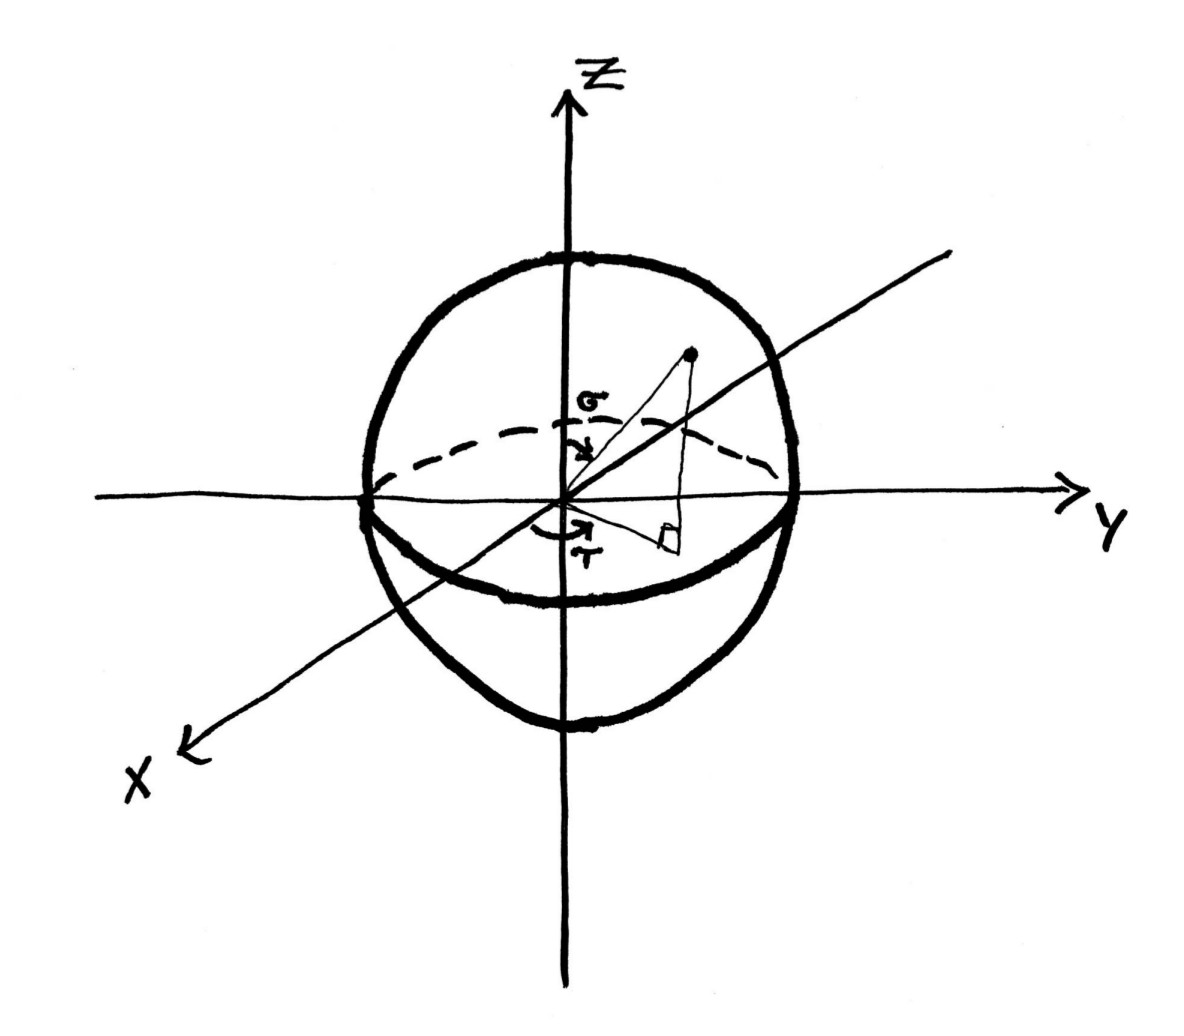
\includegraphics[width=3in]{spherePara.jpg}
\end{image}


\begin{problem}
  Show that these functions actually parameterize the $R$-sphere.
\begin{hint}
This is an exercise in ``double-containment.'' To show the one direction, show
\[
K\left(x(\sigma,\tau) ^{2}+y(\sigma,\tau) ^{2}\right) +z(\sigma,\tau)^{2} = 1
\]
for all $(\sigma,\tau)$. To show the other direction, appeal to the
diagram above.
\end{hint}
\begin{freeResponse}
  $(\subseteq)$ We will first show that the set determined by
  \[
  \left(x(\sigma,\tau), y(\sigma,\tau), z(\sigma,\tau)\right)
  \]
  lies on the surface
  \[
  K\left(x(\sigma,\tau) ^{2}+y(\sigma,\tau) ^{2}\right) +z(\sigma,\tau)^{2} = 1
  \]
  where $K=\frac{1}{R^2}>0$. Substituting we have
  $K\left(x(\sigma,\tau) ^{2}+y(\sigma,\tau) ^{2}\right)
  +z(\sigma,\tau)^{2}$
  \begin{align*}
    &=K\left((R\cdot\sin\sigma\cdot\cos\tau)^{2}+(R\cdot\sin\sigma\cdot\sin\tau)^{2}\right) +(\cos\sigma)^{2} \\
    &= \sin^2\sigma\cdot\cos^2\tau+\sin^2\sigma\sin^2\tau + \cos^2\sigma \\
    &= \sin^2\sigma(\cos^2\tau+\sin^2\tau) + \cos^2\sigma \\
    &= \sin^2\sigma + \cos^2\sigma \\
    &=1.
  \end{align*}

  $(\supseteq)$ Now we must show that every point on the surface can be obtained from
  \[
  \left(x(\sigma,\tau), y(\sigma,\tau), z(\sigma,\tau)\right).
  \]
  We see this from the diagram above. 
\end{freeResponse}
\end{problem}




If we are going to describe paths on the $R$-sphere by paths in the
$(\sigma,\tau)$-plane we are going to need to figure out the $K$-dot
product in $(\sigma,\tau)$-coordinates so that we can compute the
lengths of paths in these coordinates.

\begin{problem}
Suppose we have a curve $X$ in $K$-warped space that is a function of
$\sigma(t)$ and $\tau(t)$. So
\[
X(t) =
\begin{cases}
  x(\sigma(t),\tau(t)),\\
  y(\sigma(t),\tau(t)),\\
  z(\sigma(t),\tau(t)).\\
\end{cases}
\]
Use the chain rule to compute
\[
\dd[x]{t},\qquad \dd[y]{t}, \qquad \dd[z]{t},
\]
in terms of $\dd[\sigma]{t}$, $\dd[\tau]{t}$, $\pp[x]{\sigma}$,
$\pp[y]{\sigma}$, $\pp[z]{\sigma}$, $\pp[x]{\tau}$, $\pp[y]{\tau}$,
and $\pp[z]{\tau}$.
\begin{hint}
  Recall that if $F$ is a differentiable function of $x$, $y$, and
  $z$; and if $x$, $y$, and $z$ are all differentiable functions of
  $t$, then the chain rule states
  \[
  \dd[F]{t} = \nabla F \cdot
  \begin{bmatrix}
    \dd[x]{t} & \dd[y]{t} & \dd[z]{t}
  \end{bmatrix}^\transpose
  .
  \]
\end{hint}
\begin{freeResponse}
  Write
  \begin{align*}
    \dd[x]{t} &= \begin{bmatrix}\pp[x]{\sigma} & \pp[x]{\tau}\end{bmatrix}\cdot\begin{bmatrix}\dd[\sigma]{t} & \dd[\tau]{t}\end{bmatrix}^\transpose = \pp[x]{\sigma}\cdot\dd[\sigma]{t}+\pp[x]{\tau}\cdot\dd[\tau]{t}, \\
    \dd[y]{t} &= \begin{bmatrix}\pp[y]{\sigma} & \pp[y]{\tau}\end{bmatrix}\cdot\begin{bmatrix}\dd[\sigma]{t} & \dd[\tau]{t}\end{bmatrix}^\transpose = \pp[y]{\sigma}\cdot\dd[\sigma]{t}+\pp[y]{\tau}\cdot\dd[\tau]{t}, \\
    \dd[z]{t} &= \begin{bmatrix}\pp[z]{\sigma} & \pp[z]{\tau}\end{bmatrix}\cdot\begin{bmatrix}\dd[\sigma]{t} & \dd[\tau]{t}\end{bmatrix}^\transpose = \pp[z]{\sigma}\cdot\dd[\sigma]{t}+\pp[z]{\tau}\cdot\dd[\tau]{t}.  
  \end{align*}
\end{freeResponse}
\end{problem}

\begin{problem}
  With the same setting as in the previous problem, rewrite the result
  of your computation in matrix notation to find $D_{\mathrm{sph}}$ such
  that
\[
\begin{bmatrix}
\dd[x]{t} & \dd[y]{t} & \dd[z]{t}
\end{bmatrix}
=
\begin{bmatrix}
\frac{d\sigma}{dt} & \frac{d\tau}{dt}
\end{bmatrix}\cdot D_{\mathrm{sph}}
\]
in terms of $\pp[x]{\sigma}$, $\pp[y]{\sigma}$, $\pp[z]{\sigma}$,
$\pp[x]{\tau}$, $\pp[y]{\tau}$, and $\pp[z]{\tau}$.
\begin{freeResponse}
  \[
  D_{\mathrm{sph}} =
  \begin{bmatrix}
    \pp[x]{\sigma} & \pp[y]{\sigma} & \pp[z]{\sigma} \\
    \pp[x]{\tau}   & \pp[y]{\tau}   & \pp[z]{\tau}
  \end{bmatrix}.
  \]
\end{freeResponse}
\end{problem}


\begin{problem}
  Now find $P_\mathrm{sph}$ in terms of $K$, $\pp[x]{\sigma}$, $\pp[y]{\sigma}$,
  $\pp[z]{\sigma}$, $\pp[x]{\tau}$, $\pp[y]{\tau}$, and $\pp[z]{\tau}$
  such that
  \[
  \left(\dd[x]{t}, \dd[y]{t}, \dd[z]{t}\right)\bullet_K
  \left(\dd[x]{t}, \dd[y]{t}, \dd[z]{t}\right)
  =
  \begin{bmatrix}
    \dd[\sigma]{t} &  \dd[\tau]{t}
  \end{bmatrix}
  \cdot P_\mathrm{sph}
  \cdot
  \begin{bmatrix}
    \dd[\sigma]{t} \\  \dd[\tau]{t}
  \end{bmatrix}.
  \]
  \begin{freeResponse}
    Working from the $K$-dot product, we need that
    \begin{align*}
    \left(\dd[x]{t}, \dd[y]{t}, \dd[z]{t}\right)\bullet_K
    \left(\dd[x]{t}, \dd[y]{t}, \dd[z]{t}\right)
    &=
    \begin{bmatrix}
      \dd[x]{t} & \dd[y]{t} & \dd[z]{t}
    \end{bmatrix}
    \begin{bmatrix}
      1 & 0 & 0\\
      0 & 1 & 0\\
      0 & 0 & K^{-1}
    \end{bmatrix}
    \begin{bmatrix}
      \dd[x]{t} \\ \dd[y]{t} \\ \dd[z]{t}
    \end{bmatrix}\\
    &=
    \begin{bmatrix}
      \frac{d\sigma}{dt} & \frac{d\tau}{dt}
    \end{bmatrix}\cdot D_{\mathrm{sph}}\cdot
    \begin{bmatrix}
      1 & 0 & 0\\
      0 & 1 & 0\\
    0 & 0 & K^{-1}
    \end{bmatrix}
    \cdot
    \left(
    \begin{bmatrix}
      \frac{d\sigma}{dt} & \frac{d\tau}{dt}
    \end{bmatrix}\cdot D_{\mathrm{sph}}
    \right)^\transpose\\
    &=
    \begin{bmatrix}
      \frac{d\sigma}{dt} & \frac{d\tau}{dt}
    \end{bmatrix}\cdot D_{\mathrm{sph}}\cdot
    \begin{bmatrix}
      1 & 0 & 0\\
      0 & 1 & 0\\
    0 & 0 & K^{-1}
    \end{bmatrix}
    \cdot
    D_{\mathrm{sph}}^\transpose
    \cdot \begin{bmatrix}
      \frac{d\sigma}{dt} \\ \frac{d\tau}{dt}
    \end{bmatrix}.
  \end{align*}
    Hence
    \begin{align*}
      P_\mathrm{sph} &=
      \begin{bmatrix}
        \pp[x]{\sigma} & \pp[y]{\sigma} & \pp[z]{\sigma} \\
        \pp[x]{\tau} & \pp[y]{\tau} & \pp[z]{\tau}
      \end{bmatrix}
      \begin{bmatrix}
        1 & 0 & 0\\
        0 & 1 & 0\\
        0 & 0 & K^{-1}
      \end{bmatrix}
      \begin{bmatrix}
        \pp[x]{\sigma} & \pp[x]{\tau}\\ 
        \pp[y]{\sigma} & \pp[y]{\tau}\\
        \pp[z]{\sigma} & \pp[z]{\tau}
      \end{bmatrix}\\
      &=
      \begin{bmatrix}
        \left(\pp[x]{\sigma}\right)^2 + \left(\pp[y]{\sigma}\right)^2 + \left(\pp[z]{\sigma}\right)^2K^{-1} & \pp[x]{\sigma}\pp[x]{\tau} + \pp[y]{\sigma}\pp[y]{\tau} + \pp[z]{\sigma}\pp[z]{\tau} K^{-1}\\
        \pp[x]{\sigma}\pp[x]{\tau} + \pp[y]{\sigma}\pp[y]{\tau} + \pp[z]{\sigma}\pp[z]{\tau} K^{-1}       & \left(\pp[x]{\tau}\right)^2 + \left(\pp[y]{\tau}\right)^2 + \left(\pp[z]{\tau}\right)^2K^{-1}
      \end{bmatrix}.
    \end{align*}
  \end{freeResponse}
\end{problem}


\begin{problem}
  Set
  \begin{align*}
    x(\sigma,\tau) &=R\cdot \sin\sigma\cdot \cos \tau,\\
    y(\sigma,\tau) &=R\cdot \sin\sigma\cdot \sin\tau,\\
    z(\sigma,\tau) &=\cos \sigma,
  \end{align*}
  and show that $P_\mathrm{sph}$ from the problem above is
  \[
  P_\mathrm{sph} =
  \begin{bmatrix}
    R^2 & 0 \\
    0 & R^2\cdot\sin^2 \sigma
  \end{bmatrix}.
  \]
  \begin{freeResponse}
    Write
    \[
    \begin{split}
      \pp[x]{\sigma} &= R\cdot \cos\sigma\cdot \cos \tau, \\
      \pp[y]{\sigma} &= R\cdot \cos\sigma\cdot \sin\tau,\\
      \pp[z]{\sigma} &= -\sin\sigma,
    \end{split}
    \qquad
    \begin{split}
      \pp[x]{\tau} &= -R\cdot \sin\sigma\cdot \sin \tau,\\
      \pp[y]{\tau} &= R\cdot \sin\sigma\cdot \cos\tau,\\
      \pp[z]{\tau} &= 0. 
    \end{split}
    \]
    Now we see $\left(\pp[x]{\sigma}\right)^2 + \left(\pp[y]{\sigma}\right)^2 + \left(\pp[z]{\sigma}\right)^2K^{-1}$
    \begin{align*}
      &= \left(R\cdot \cos\sigma\cdot \cos \tau \right)^2 + \left(R\cdot \cos\sigma\cdot \sin\tau\right)^2 + \left(-\sin\sigma\right)^2K^{-1}\\
      &= R^2\cdot \cos^2\sigma\cdot \cos^2 \tau + R^2\cdot \cos^2\sigma\cdot \sin^2\tau + R^2 \sin^2\sigma \\
      &= R^2\cdot \cos^2\sigma\left(\cos^2 \tau + \sin^2\tau\right) + R^2 \sin^2\sigma \\
      &= R^2\left(\cos^2\sigma + \sin^2\sigma\right) \\
      &= R^2.
    \end{align*}
    That $\pp[x]{\sigma}\pp[x]{\tau} + \pp[y]{\sigma}\pp[y]{\tau} + \pp[z]{\sigma}\pp[z]{\tau} K^{-1}$
    \begin{align*}
      &= -R^2\cdot \cos\sigma\cdot \cos \tau \cdot \sin\sigma\cdot \sin \tau + R^2\cdot \cos\sigma\cdot \cos \tau \cdot \sin\sigma\cdot \sin \tau\\
      &= 0.
    \end{align*}
    And finally that $\left(\pp[x]{\tau}\right)^2 + \left(\pp[y]{\tau}\right)^2 + \left(\pp[z]{\tau}\right)^2K^{-1}$
     \begin{align*}
       &= \left(-R\cdot \sin\sigma\cdot \sin \tau \right)^2 + \left( R\cdot \sin\sigma\cdot \cos\tau \right)^2 \\
       &= R^2\cdot \sin^2\sigma\cdot \sin^2 \tau + R^2\cdot \sin^2\sigma\cdot \cos^2\tau \\
       &= R^2\cdot \sin^2\sigma\left(\sin^2 \tau + \cos^2\tau\right) \\
       &= R^2\cdot \sin^2\sigma.
     \end{align*}
     Hence
     \[
     P_\mathrm{sph} =
  \begin{bmatrix}
    R^2 & 0 \\
    0 & R^2\cdot\sin^2 \sigma
  \end{bmatrix}.
     \]
  \end{freeResponse}
\end{problem}

\begin{definition}
  Let $V_\mathrm{sph}$ and $W_\mathrm{sph}$ be a vectors in
  $(\sigma,\tau)$-coordinates originating at the same
  $(\sigma,\tau)$-coordinate. Define
  \[
  V_\mathrm{sph} \bullet_\mathrm{sph} W_\mathrm{sph} = V_\mathrm{sph} \cdot P_\mathrm{sph} \cdot W_\mathrm{sph}^\transpose
  \]
  where
  \[
  P_\mathrm{sph} =
  \begin{bmatrix}
    R^2 & 0 \\
    0 & R^2\cdot\sin^2 \sigma
  \end{bmatrix}
  \]
  and $\sigma$ is determined by the coordinate that the vectors
  originate from.
\end{definition}


Now notice that you can write a path on the $R$-sphere by giving a path
$\left( \sigma(t),\tau(t)\right)$ in the $(\sigma,\tau)$-plane. In
fact, you can use $\sigma$ as the parameter, and just write
\[
\left(\sigma,\tau(\sigma)\right)
\]
where $\tau$ is a function of $\sigma$. To write a path that starts at
the North Pole, just write%
\[
\left(\sigma,\tau(\sigma)\right), \qquad 0\leq\sigma\leq\varepsilon
\]
and demand that
\[
\tau(0) =0.
\]
If you want the path to end on the plane $y=\hat{y}=0$, demand
additionally that
\[
\tau(\varepsilon) =0.
\]

%% \begin{problem}
%% \begin{enumerate}
%% \item Referring to $\left(\ref{133}\right)$ compute the $2\times3$
%%   matrix
%% \[
%% D_{sph}=\left(
%% \begin{array}
%% [c]{ccc}%
%% \frac{\partial x}{\partial \sigma} & \frac{\partial y}{\partial \sigma} & \frac{\partial z}{\partial \sigma}\\
%% \frac{\partial x}{\partial \tau} & \frac{\partial y}{\partial \tau} & \frac{\partial z}{\partial \tau}%
%% \end{array}
%% \right)  .
%% \]


%% \item  Show that, if a path in $K$-geometry is given by a path $\left(
%% \sigma\left(  t\right)  ,\tau\left(  t\right)  \right)  $ in the $\left(
%% \sigma,\tau\right)  $-plane,%
%% \[
%% \left(  \frac{dx}{dt},\frac{dy}{dt},\frac{dz}{dt}\right)  =\left(
%% \frac{d\sigma}{dt},\frac{d\tau}{dt}\right)  \cdot D_{sph}.
%% \]


%% \item For two paths in $K$-geometry given by paths $\left(  \sigma_{1}\left(
%% t\right)  ,\tau_{1}\left(  t\right)  \right)  $ and $\left(  \sigma_{2}\left(
%% t\right)  ,\tau_{2}\left(  t\right)  \right)  $ in the $\left(  \sigma
%% ,\tau\right)  $-plane, use a) and b) to show that
%% \begin{gather*}
%% \left(  \frac{d\hat{x}_{1}}{dt},\frac{d\hat{y}_{1}}{dt},\frac{d\hat{z}_{1}%
%% }{dt}\right)  \cdot\left(  \frac{d\hat{x}_{2}}{dt},\frac{d\hat{y}_{2}}{dt}%
%% ,\frac{d\hat{z}_{2}}{dt}\right)  ^{t}=\\
%% \left(  \frac{dx_{1}}{dt},\frac{dy_{1}}{dt},\frac{dz_{1}}{dt}\right)
%% \cdot\left(
%% \begin{array}
%% [c]{ccc}%
%% 1 & 0 & 0\\
%% 0 & 1 & 0\\
%% 0 & 0 & K^{-1}%
%% \end{array}
%% \right)  \cdot\left(  \frac{dx_{2}}{dt},\frac{dy_{2}}{dt},\frac{dz_{2}}%
%% {dt}\right)  ^{t}=\\
%% \left(  \frac{d\sigma_{1}}{dt},\frac{d\tau_{1}}{dt}\right)  \cdot
%% \left({\tiny
%% \begin{array}{cc}
%%  \frac{\cos \left(\sigma _1\right) \cos \left(\sigma _2\right) \cos
%%    \left(\tau _1-\tau _2\right)+\sin \left(\sigma _1\right) \sin
%%    \left(\sigma _2\right)}{K} & \frac{\sin \left(\sigma _2\right)
%%    \cos \left(\sigma _1\right) \sin \left(\tau _1-\tau
%%    _2\right)}{K} \\
%%  -\frac{\sin \left(\sigma _1\right) \cos \left(\sigma _2\right)
%%    \sin \left(\tau _1-\tau _2\right)}{K} & \frac{\sin \left(\sigma
%%    _1\right) \sin \left(\sigma _2\right) \cos \left(\tau _1-\tau
%%    _2\right)}{K} \\
%% \end{array}}
%% \right)
%% \cdot\left(  \frac{d\sigma_{2}}{dt},\frac{d\tau_{2}}{dt}\right)  ^{t}%
%% \end{gather*}

%% \item Explain why the definition%
%% \[
%% \left(  \frac{d\sigma_{1}}{dt},\frac{d\tau_{1}}{dt}\right)  \bullet
%% _{sph}\left(  \frac{d\sigma_{2}}{dt},\frac{d\tau_{2}}{dt}\right)  =
%% \]
%% \[
%% \left(
%% \frac{d\sigma_{1}}{dt},\frac{d\tau_{1}}{dt}\right)  \cdot
%% \left({\tiny
%% \begin{array}{cc}
%%  \frac{\cos \left(\sigma _1\right) \cos \left(\sigma _2\right) \cos
%%    \left(\tau _1-\tau _2\right)+\sin \left(\sigma _1\right) \sin
%%    \left(\sigma _2\right)}{K} & \frac{\sin \left(\sigma _2\right)
%%    \cos \left(\sigma _1\right) \sin \left(\tau _1-\tau
%%    _2\right)}{K} \\
%%  -\frac{\sin \left(\sigma _1\right) \cos \left(\sigma _2\right)
%%    \sin \left(\tau _1-\tau _2\right)}{K} & \frac{\sin \left(\sigma
%%    _1\right) \sin \left(\sigma _2\right) \cos \left(\tau _1-\tau
%%    _2\right)}{K} \\
%% \end{array}}
%% \right)
%% \cdot\left(  \frac{d\sigma_{2}}{dt},\frac{d\tau_{2}}{dt}\right)  ^{t}%
%% \]
%% allows us to compute the dot product of two tangent vectors to the $R$-sphere
%% in Euclidean space if we just know the values of the two corresponding vectors
%% in the $\left(  \sigma,\tau\right)  $-plane.
%% \end{enumerate}
%% \end{problem}
 Now given a path on the $R$-sphere
 \[
 \left(\sigma,\tau(\sigma)\right),\qquad0\leq\sigma \leq\varepsilon
 \]
 with
 \[
 \tau\left(  0\right)  =0.
 \]
 and%
 \[
 \tau\left(  \varepsilon\right)  =0
 \]
 its length is given by the formula%
\[
L=\int_{0}^{\varepsilon} \sqrt{\left(1,\dd[\tau]{\sigma}\right)\bullet_\mathrm{sph} \left(1,\dd[\tau]{\sigma}\right)}\d\sigma.
\]

\begin{problem}
  Prove that the shortest path on the $R$-sphere from the North Pole
  \[
  N=\left( R\cdot \sin 0\cdot  \cos 0,R\cdot \sin  0\cdot \sin 0,\cos
  0\right)
  \]
  to a point
  \[
  (x,y,z)=\left(R\cdot \sin \varepsilon,0,\cos \varepsilon\right)
  \]
  is the path lying in the plane $y=0$.
  \begin{hint}
    Note that the following expression is always positive:
    \[
    1+\sin ^{2}\sigma\cdot \left(\frac{d\tau }{d\sigma}\right)^{2}.
    \]
    When is it minimal?
  \end{hint}

  \begin{freeResponse}
    Write
    \begin{align*}
    L  &=\int_{0}^{\varepsilon} \sqrt{\left(1,\dd[\tau]{\sigma}\right)\bullet_\mathrm{sph} \left(1,\dd[\tau]{\sigma}\right)}\d\sigma\\
    &= \int_{0}^{\varepsilon} \sqrt{
      \begin{bmatrix} 1 & \dd[\tau]{\sigma}
      \end{bmatrix} \cdot P_\mathrm{sph}\cdot
      \begin{bmatrix} 1 & \dd[\tau]{\sigma}
      \end{bmatrix}^\transpose}\d\sigma \\
    &= \int_{0}^{\varepsilon} \sqrt{
      \begin{bmatrix} 1 & \dd[\tau]{\sigma}
      \end{bmatrix}
      \begin{bmatrix}
        R^2 & 0 \\
        0 & R^2\cdot\sin^2 \sigma
      \end{bmatrix}
      \begin{bmatrix} 1 \\ \dd[\tau]{\sigma}
    \end{bmatrix}}\d\sigma \\
    &= \int_{0}^{\varepsilon} \sqrt{
      R^2+R^2\sin^{2}\sigma\cdot \left(\frac{d\tau }{d\sigma}\right)^{2}
    }\d\sigma \\
    &= R\int_{0}^{\varepsilon} \sqrt{
      1+\sin^{2}\sigma\cdot \left(\frac{d\tau }{d\sigma}\right)^{2}
    }\d\sigma.
    \end{align*}
   Since $\sin^{2}\sigma$ is is positive for almost all $\sigma\in[
     0,\varepsilon] $, $L$ is minimal only when
   $\frac{d\tau}{d\sigma}$ is identically $0$. But this means that
   $\tau\left( \sigma\right) $ is a constant function. Since
   $\tau\left( 0\right) =0$, this means that $\tau\left( \sigma\right)
   $ is identically $0$. Hence our path is determined by
   \begin{align*}
     x(\sigma,\tau) &=R\cdot \sin\sigma,\\
     y(\sigma,\tau) &=0,\\
     z(\sigma,\tau) &=\cos \sigma,
   \end{align*}
   and this corresponds to a circular arc embedded in the plane
   $y=\hat{y}=0$.
  \end{freeResponse}

\end{problem}









\section{Shortest path between any two points}

We next prove the theorem that shows that shortest path on the surface
of the Earth from Rio de Janeiro to Los Angeles is the one cut on the
surface of the Earth by the plane that passes through the center of
the Earth and through Rio and through Los Angeles. That is usually the
route an airplane would take when flying between the two cities.


\begin{theorem}
Given any two points $X_{1}=\left(x_{1},y_{1},z_{1}\right) $ and
$X_{2}=\left(x_{2},y_{2},z_{_{2}}\right) $ in $K$-geometry, the
shortest path between the two points is the path cut out by the set
\[
K\left(  x^{2}+y^{2}\right)  +z^{2}=1
\]
and the plane containing $(0,0,0)$, $X_{1}$, and $X_{2}$.
\end{theorem}

\begin{problem}
  Explain in words how to prove this theorem by using the $K$-rigid
  motions
  \[
  M_\theta=
  \begin{bmatrix}
    \cos\theta & \sin\theta & 0\\
    -\sin\theta & \cos\theta & 0\\
    0 & 0 & 1
  \end{bmatrix}
  \qquad\text{and}\qquad
  N_\psi=
  \begin{bmatrix}
    \cos\psi & 0 & R^{-1}\cdot\sin\psi\\
    0 & 1 & 0\\
    -R\cdot\sin\psi & 0 & \cos\psi
  \end{bmatrix}.
  \]
  \begin{hint}
    $M_\theta$ is a $K$-rigid motion that rotates around the $z$-axis and
    $N_\psi$ is a $K$-rigid motion that rotates around the $y$-axis.
  \end{hint}
  \begin{hint}
    You should apply \textit{two} $K$-rigid motions of the form
    $M_\theta$ (for different angles) and one $K$-rigid motion of the
    form $N_\psi$, though not necessarily in that order!
  \end{hint}
  \begin{freeResponse}
    Given $X_1$ and $X_2$, we may instead consider $X_1\cdot M_\theta$
    and $X_2\cdot M_\theta$ where $\theta$ is chosen so that $X_1\cdot
    M_\theta$ is in the plane $y=0$.

    Next consider $X_1\cdot M_\theta\cdot N_\psi$ and $X_2\cdot
    M_\theta\cdot N_\psi$ where $\psi$ is chosen so that $X_1\cdot
    M_\theta\cdot N_\psi$ is at the North Pole.

    Finally consider $X_1\cdot M_\theta\cdot N_\psi\cdot M_\varphi$
    and $X_2\cdot M_\theta\cdot N_\psi\cdot M_\varphi$ where $\varphi$
    is chosen so that $X_1\cdot M_\theta\cdot N_\psi\cdot M_\varphi$
    is at the North Pole and $X_2\cdot M_\theta\cdot N_\psi\cdot
    M_\varphi$ is in the plane $y=0$.

    Now by our previous work, the shortest path between $X_1\cdot
    M_\theta\cdot N_\psi\cdot M_\varphi$ and $X_2\cdot M_\theta\cdot
    N_\psi\cdot M_\varphi$ is the great circular arc in the plane
    $y=0$. Applying $M_\varphi^{-1}\cdot N_\psi^{-1}\cdot
    M_\theta^{-1}$ to our ``moved'' points will move them back again,
    and the shortest path is the transformed great circular arc.
  \end{freeResponse}
\end{problem}

%% \begin{theorem}
%% Given any two points $X_{1}=\left(x_{1},y_{1},z_{1}\right) $ and
%% $X_{2}=\left(x_{2},y_{2},z_{_{2}}\right) $ in $K$-geometry, the
%% shortest path between the two points is the path cut out by the two
%% equations
%% \[
%% K\left(  x^{2}+y^{2}\right)  +z^{2}=1
%% \]
%% \begin{equation}
%% \left\vert \left(
%% \begin{array}
%% [c]{ccc}%
%% x & y & z\\
%% x_{1} & y_{1} & z_{1}\\
%% x_{2} & y_{2} & z_{2}%
%% \end{array}
%% \right)  \right\vert =0, \label{63}%
%% \end{equation}
%% that is, the plane containing $\left(  0,0,0\right)  $ and $X_{1}$ and $X_{2}$.
%% \end{theorem}

%% \begin{proof}
%% By a previous problem there is a $K$-rigid motion $M$ that takes
%% $X_{1}$ to the North Pole $N$ and $X_{2}$ to $\left(
%% K^{-1/2}\sin\varepsilon,0,\cos\varepsilon \right) $ for some
%% $\varepsilon$. That is%
%% \[
%% X_{2}\cdot M=\left(  R\cdot \sin \varepsilon
%% ,0,\cos \varepsilon\right)
%% \]
%% for some $\varepsilon$ since all points in $K$-geometry with \underline{$y$%
%% }$=0$ can be written as $\left(  R\cdot \sin %
%% \varepsilon,0,\cos \varepsilon\right)  $ for some $\varepsilon$. But%
%% \begin{align*}
%% \left\vert \left(
%% \begin{array}
%% [c]{ccc}%
%% \underline{x} & \underline{y} & \underline{z}\\
%% 0 & 0 & 1\\
%% K^{-1/2}\sin\varepsilon & 0 & \cos\varepsilon
%% \end{array}
%% \right)  \right\vert  &  =\left\vert \left(
%% \begin{array}
%% [c]{ccc}%
%% x & y & z\\
%% x_{1} & y_{1} & z_{1}\\
%% x_{2} & y_{2} & z_{2}%
%% \end{array}
%% \right)  \cdot M\right\vert \\
%% &  =\left\vert \left(
%% \begin{array}
%% [c]{ccc}%
%% x & y & z\\
%% x_{1} & y_{1} & z_{1}\\
%% x_{2} & y_{2} & z_{2}%
%% \end{array}
%% \right)  \right\vert \cdot\left\vert M\right\vert =0,
%% \end{align*}
%% Since $\left\vert M\right\vert \neq0$ and $K^{-1/2}\sin\varepsilon\neq0$ if
%% $\varepsilon<\pi$, $\left(  x,y,z\right)  $ lies in the plane $\left(
%% \ref{63}\right)  $ if and only if
%% \[
%% \underline{y}=0.
%% \]
%% Since $M$ is a $K$-rigid motion it must take the shortest path from $X_{1}$ to
%% $X_{2}$ to the shortest path from $X_{1}\cdot M=N$ to $X_{2}\cdot M=\left(
%% R\cdot \sin \varepsilon,0,\cos %
%% \varepsilon\right)  $. But we already know that the shortest path from
%% $X_{1}\cdot M$ to $X_{2}\cdot M$ is the one cut out by the plane $y=0$. But
%% that path comes from the path cut out by the plane given by equation $\left(
%% \ref{63}\right)  $. This path is called the \textit{great circular arc}
%% between $X_{1}$ and $X_{2}$.
%% \end{proof}

\begin{definition}
A \dfn{line} in spherical geometry will be a curve that extends
infinitely in each direction and has the property that, given any two
points $X_{1}$ and $X_{2}$ on the path, the shortest path between
$X_{1}$ and $X_{2}$ lies along that curve.

Lines in spherical geometry are usually called great circles on the
$R$-sphere. They are the intersections of the $R$-sphere with planes
through $(0,0,0)$.
\end{definition}

%% Letting $X_{2}$ approach $X_{1}$ along the great circular arc joining $X_{1}$
%% and $X_{2}$ we see that the solution set to equation $\left(  \ref{63}\right)
%% $ does not change. Taking a limit as $X_{2}$ approaches $X_{1}$, this set can
%% also be expressed as the solution set of the equation%
%% \[
%% \left\vert \left(
%% \begin{array}
%% [c]{ccc}%
%% x & y & z\\
%% x_{1} & y_{1} & z_{1}\\
%% a_{1} & b_{1} & c_{1}%
%% \end{array}
%% \right)  \right\vert =0
%% \]
%% where $\left(  a_{1},b_{1},c_{1}\right)  $ is a tangent vector at the point
%% $X_{1}$ pointing in the direction of $X_{2}.$

\section{The spherical Pythagorean Theorem}

To start we need some basic facts about lengths of lines in spherical
geometry.

\begin{problem}
  Given a line in spherical geometry lying entire in the plane $y=0$,
  \begin{align*}
    x(\varepsilon) &= R\cdot\sin\varepsilon,\\
    y(\varepsilon) &= 0,\\
    z(\varepsilon) &= \cos\varepsilon,
  \end{align*}
  show that its length is exactly $R\cdot \varepsilon$.
  \begin{hint}
    Use a previous problem.
  \end{hint}
  \begin{freeResponse}
    By a previous problem the length of this line is given by
    \[
    L=R \cdot \int_{0}^{\varepsilon} 1 \d\sigma = R\cdot\varepsilon.
    \]
  \end{freeResponse}
\end{problem}

\begin{problem}
  Explain in words how to prove that given two points on $R$-sphere,
  say $X_A$ and $X_B$, the length of the spherical line connecting them
  is given by
  \[
  R\cdot \varepsilon = R\cdot\arccos\left(\frac{X_A\bullet_K X_B}{|X_A|_K\cdot |X_B|_K}\right).
  \]
  by using the $K$-rigid motions
  \[
   M_\theta=
  \begin{bmatrix}
    \cos\theta & \sin\theta & 0\\
    -\sin\theta & \cos\theta & 0\\
    0 & 0 & 1
  \end{bmatrix}
  \qquad\text{and}\qquad
  N_\psi=
  \begin{bmatrix}
    \cos\psi & 0 & R^{-1}\cdot\sin\psi\\
    0 & 1 & 0\\
    -R\cdot\sin\psi & 0 & \cos\psi
  \end{bmatrix}.
  \]
  \begin{freeResponse}
    The problem is essentially the same as a previous problem. Hence one must consider
    \[
    X_A\cdot M_\theta\cdot N_\psi\cdot M_\varphi \qquad\text{and}\qquad
    X_B\cdot M_\theta\cdot N_\psi\cdot M_\varphi
    \]
    where $\theta$, $\psi$, and $\varphi$ are chosen to place $X_A$ on
    the North Pole and $X_B$ in the plane $y=0$.

    Now we know the distance between the points to be $R\cdot
    \varepsilon$. Since $K$-rigid motions preserve distance and angle,
    this completes the proof.
  \end{freeResponse}
\end{problem}


We will now give the spherical analogue of the Pythagorean Theorem.

\begin{theorem}[Spherical Pythagorean Theorem]
  If $\triangle X_AX_BX_C$ is a right triangle on the $R$-sphere with right
  angle $\angle X_AX_CX_B$, and side $a$ opposite $X_A$, $b$ opposite $X_B$,
  and $c$ opposite $X_C$, then
  \[
  \cos\left(\frac{c}{R}\right)=\cos\left(\frac{a}{R}\right)\cos\left(\frac{b}{R}\right).
  \]
\end{theorem}

Let's see why this theorem is true.  We may via $K$-rigid motions
place the triangle so that $X_C$ is at the North Pole, $X_A$ is in the
plane $y=0$, and $X_B$ is in the plane $x=0$ (note $X_A$ and $X_B$ may
be switched---if this is the case, simply rename them). In this case,
\begin{align*}
  X_A &= (R\cdot \sin\alpha, 0, \cos\alpha),\\
  X_B &= (0, R\cdot \sin \beta, \cos\beta).
\end{align*}
\begin{image}
  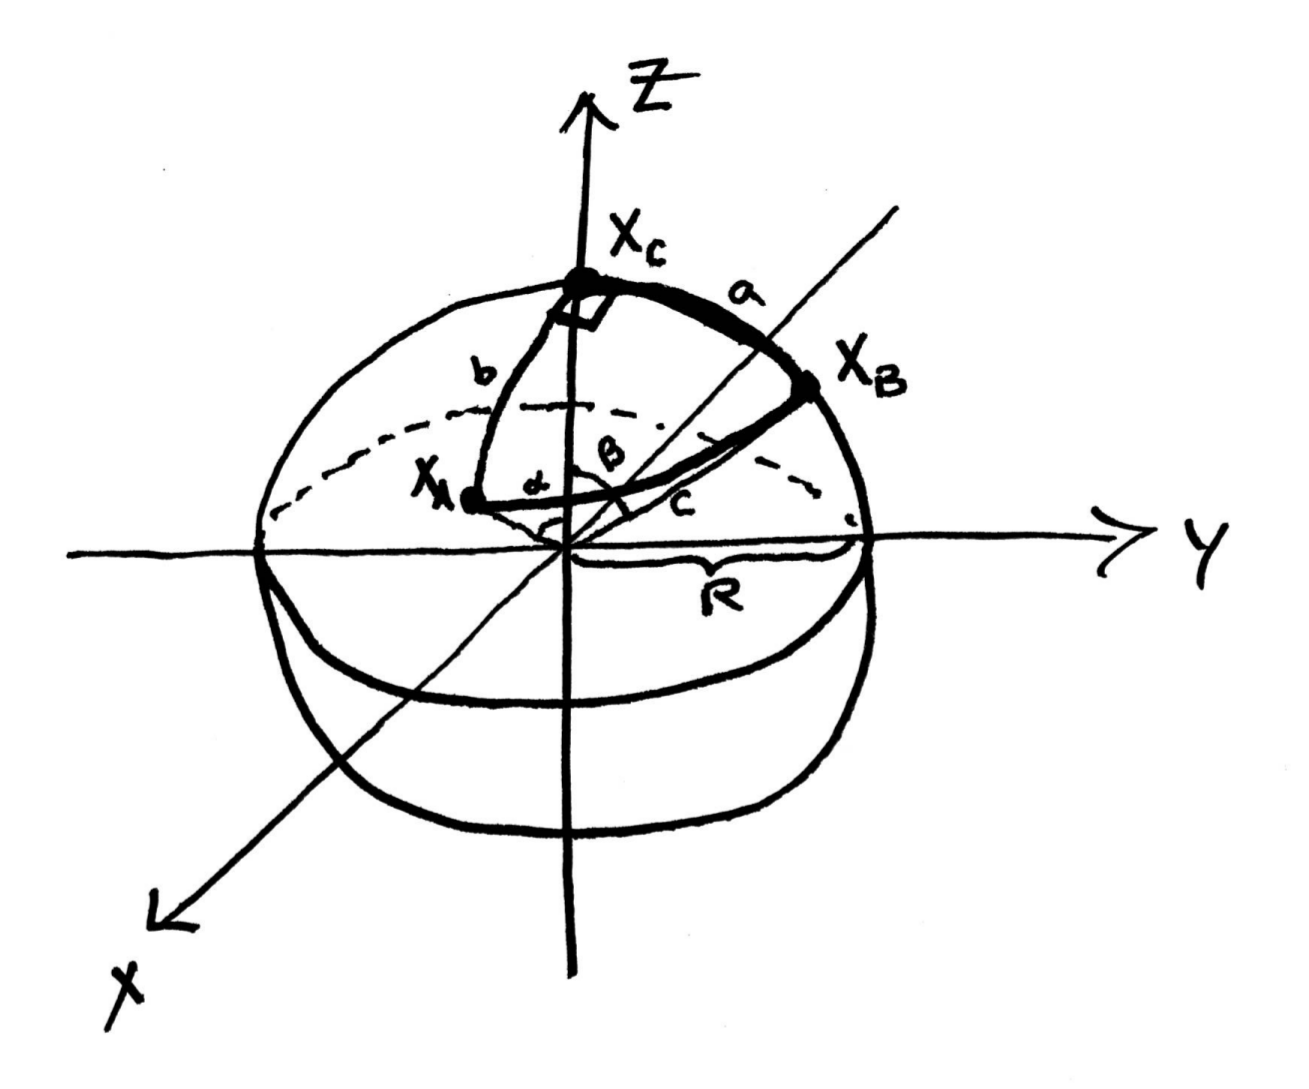
\includegraphics[width=4in]{sphPythag.png}
\end{image}
Hence the length of side $b$ is $R\cdot\alpha$. Using a rigid motion of the form
\[
M_\theta=
\begin{bmatrix}
  \cos\theta & \sin\theta & 0\\
  -\sin\theta & \cos\theta & 0\\
  0 & 0 & 1
\end{bmatrix}
\]
when $\theta = \pi/2$ we see that the length of side $a$ is $R\cdot
\beta$. Set
\[
\gamma = \arccos\left(\frac{X_A\bullet_K X_B}{|X_A|_K\cdot |X_B|_K}\right).
\]
Since we are working on the $R$-sphere,
\begin{align*}
  R^2\cdot \cos \gamma &= X_A\bullet_K X_B\\
  &=
  \begin{bmatrix}
    R\cdot \sin\alpha &  0 & \cos\alpha
  \end{bmatrix}
    \begin{bmatrix}
      1 & 0 & 0\\
      0 & 1 & 0\\
      0 & 0 & R^2
    \end{bmatrix}
    \begin{bmatrix}
      0\\
      R\cdot\sin\beta\\
      \cos\beta
    \end{bmatrix}\\
   &=R^2 \cdot \cos\alpha \cdot \cos\beta.
  \end{align*}
\begin{problem}
  Explain how to progress from the fact that
  \[
  R^2\cdot \cos \gamma = R^2 \cdot \cos\alpha \cdot \cos\beta.
  \]
  to the conclusion of the theorem
  \[
  \cos\left(\frac{c}{R}\right)=\cos\left(\frac{a}{R}\right)\cos\left(\frac{b}{R}\right).
  \]
  \begin{freeResponse}
    As we have seen
    \[
    \begin{split}
      R\cdot \alpha &= a,\\
      R\cdot \beta  &= b,\\
      R\cdot \gamma &= c,
    \end{split}
    \qquad\text{so}\qquad
    \begin{split}
      \alpha &= \frac{a}{R},\\
      \beta  &= \frac{b}{R},\\
      \gamma &= \frac{c}{R},
    \end{split}
    \]
    and hence
    \[
    \cos\left(\frac{c}{R}\right)=\cos\left(\frac{a}{R}\right)\cos\left(\frac{b}{R}\right).
    \]
  \end{freeResponse}
\end{problem}


\begin{problem}
  Use the Taylor series expansion of $\cos(x)$ centered around $x=0$,
  \[
  \cos(x) = 1 - \frac{x^2}{2!} + \frac{x^4}{4!} - \frac{x^6}{6!} + \cdots
  \]
to show that for ``small'' triangles, the spherical Pythagorean
Theorem reduces to the euclidean Pythagorean Theorem, meaning
\[
c^2 \approx a^2+b^2.
\]
\begin{freeResponse}
  If
  \[
  \cos\left(\frac{c}{R}\right)=\cos\left(\frac{a}{R}\right)\cos\left(\frac{b}{R}\right),
  \]
  then we may replace each cosine with its Taylor series expansion
  \[
  1 - \frac{\left(\frac{c}{R}\right)^2}{2!} + \frac{\left(\frac{c}{R}\right)^4}{4!} - \frac{\left(\frac{c}{R}\right)^6}{6!} + \cdots
  \]
  \[
  =\left(
  1 - \frac{\left(\frac{a}{R}\right)^2}{2!} + \frac{\left(\frac{a}{R}\right)^4}{4!} - \frac{\left(\frac{a}{R}\right)^6}{6!} + \cdots
  \right)
  \left(
  1 - \frac{\left(\frac{b}{R}\right)^2}{2!} + \frac{\left(\frac{b}{R}\right)^4}{4!} - \frac{\left(\frac{b}{R}\right)^6}{6!} + \cdots
  \right).
  \]
  Expanding this out, and discarding higher-order terms (as they will
  go to zero when $R$ is large relative to $a$, $b$, and $c$) we find
  \[
  \frac{-1}{2}\left(\frac{c}{R}\right)^2 = \frac{-1}{2}\left(\frac{a}{R}\right)^2+\frac{-1}{2}\left(\frac{b}{R}\right)^2.
  \]
  Multiplying both sides of the equation by $-2R^2$, we see that for a
  ``small'' right triangle on a sphere,
  \[
  c^2 \approx a^2 +b^2.
  \]
\end{freeResponse}
\end{problem}


\begin{problem}
Summarize the results from this section. In particular, indicate which
results follow from the others.
\begin{freeResponse}
\end{freeResponse}
\end{problem}




\end{document}
